\documentclass[10pt]{article}
\usepackage{fullpage}
\usepackage{amsmath,amsfonts,amsthm}
\usepackage{graphicx}
\usepackage{multirow}
\usepackage{hhline}

%\graphicspath{{./imgs/} {./imgs/Q1/} {./imgs/Q2/}}

% these are compressed lists to help fit into a 1 page limit
\newenvironment{enumerate*}%
  {\vspace{-2ex} \begin{enumerate} %
     \setlength{\itemsep}{-1ex} \setlength{\parsep}{0pt}}%
  {\end{enumerate}}
 
\newenvironment{itemize*}%
  {\vspace{-2ex} \begin{itemize} %
     \setlength{\itemsep}{-1ex} \setlength{\parsep}{0pt}}%
  {\end{itemize}}
 
\newenvironment{description*}%
  {\vspace{-2ex} \begin{description} %
     \setlength{\itemsep}{-1ex} \setlength{\parsep}{0pt}}%
  {\end{description}}

\DeclareMathOperator*{\E}{\mathbb{E}}
\let\Pr\relax
\DeclareMathOperator*{\Pr}{\mathbb{P}}

\newcommand{\inprod}[1]{\left\langle #1 \right\rangle}
\newcommand{\eqdef}{\mathbin{\stackrel{\rm def}{=}}}

\newtheorem{theorem}{Theorem}
\newtheorem{lemma}{Lemma}

\author{Jacob Clouse}
\title{Spring 2023 - ICSI 526\\Homework $2$}

\begin{document}

\maketitle
\tableofcontents
\vspace{0.2in}
\section{Youtube Video Link:}
\noindent Watch my video on my HW2 submission at:  \textbf{https://www.youtube.com/watch?v=gN8QLL6h-Q0}
\vspace{0.2in}
\section{My CBC \& OFB Mode Implementations:}
\noindent There are two separate AES files included: One contains my code for CBC mode and the other contains my code for OFB mode. I couldn't get them to work together inside of the same file so I had to split them out into different programs. I ended up using the provided AES\_Demo.java file for the GUI of both implementations as I did not need to change anything in that file to implement my code and it was not specified that I could not use it as is. NOTE: This program was mainly coded on a Linux Mint machine using BASH to compile and Git/Github to host my code (using a private git repo). Running CBC and OFB modes are almost identical, but I have included instructions for both here for the sake of completeness. 
\vspace{0.2in}
\\
\subsection{How to Compile \& Run CBC Mode: } 
\begin{enumerate}
	\item Make sure you have a working copy of the Java JDK and a text editor on your machine (I use VS Code because of the built in terminal).
	
	\item Make sure you have x3 test files of 2000 characters each (with 0\%, 25\% and 50\% duplication respectively).
	
	\item Make a copy of the \textbf{CBC} folder I have provided and cd into it with your terminal. The ONLY two items you should have inside are the \textbf{AES.java} and \textbf{AES\_Demo.java} files (the demo is required to run this program).
	
	\item You can compile the program by using the syntax: \begin{verbatim} javac AES_Demo.java AES.java \end{verbatim}
	This should create a several class files within the \textbf{CBC} folder, including a \text{AES\_Demo.class} file.
	
	\item Now you can run this file using the syntax: 
	\begin{verbatim} java AES_Demo \end{verbatim} 
	If successful, a window should pop up titled \textbf{Jacob Clouse CBC Demo:} that will allow you to select your sample data files. 
	
	\item You can use the \textit{Browse Files} button and navigate to the first test file on your computer. \textbf{DO NOT} select either 'Preserve Image Header' or 'Reduced AES - 4 rounds'. 
	
	\item You can select where you want the encrypted output file to go using the \textbf{Choose Save Directory} button. \textbf{NOTE:} On linux, I have noticed that the output file sometimes will be stored in the parent directory of the folder you initially selected. 
	
	\item Finally, you can click \text{Begin AES} and it will encrypt your file (there is no decryption in this file, so the 'Encryption Time' and  'Decryption Time' fields may be blank). You now have your encrypted output and you repeat the process to encrypt other files as you please.
	
	\subsection{CBC Coding \& Observations: }
	\noindent I mainly made changes to the encrypt() function in the AES.java file, and almost didn't touch the AES\_Demo.file (except for updating the title). \\
	My main modifications consisted of adjusting the data that was fed into the encryptBloc() function (starting around line 315 in my code). Basically, I wanted generate an IV of the block size length to be used with the encryptBloc() function. Then we could then XOR this IV with our bloc before it is fed into the for loop for encryption. After we have encrypted our bloc, we take the result and overwrite our initial IV vector with it to be used with the next bloc.\\
	\newline
	\noindent I found that the IOC results were the most interesting vs the previous ECB implementation. For ECB, you could clearly see that a higher IOC existed between the samples (the more shared characters, the higher the IOC). But this was not the case with my CBC mode, the results basically held the same IOC regardless of initial shared content.

\end{enumerate}
\vspace{0.2in}
\subsection{How to Compile \& Run OFB Mode: } 
\begin{enumerate}
	\item Make sure you have a working copy of the Java JDK and a text editor on your machine (I use VS Code because of the built in terminal). If you have already run CBC mode, then you should be all set.
	
	\item Make sure you have x3 test files of 2000 characters each (with 0\%, 25\% and 50\% duplication respectively). Again, you can just reuse the same input files from CBC mode. 
	
	\item Make a copy of the \textbf{OFB} folder I have provided and cd into it with your terminal. The ONLY two items you should have inside are the \textbf{AES.java} and \textbf{AES\_Demo.java} files (the demo is required to run this program).
	
	\item You can compile the program by using the syntax: \begin{verbatim} javac AES_Demo.java AES.java \end{verbatim}
	This should create a several class files within the \textbf{OFB} folder, including a \text{AES\_Demo.class} file.
	
	\item Now you can run this file using the syntax: 
	\begin{verbatim} java AES_Demo \end{verbatim} 
	If successful, a window should pop up titled \textbf{Jacob Clouse OFB Demo:} that will allow you to select your sample data files. 
	
	\item You can use the \textit{Browse Files} button and navigate to the first test file on your computer. \textbf{DO NOT} select either 'Preserve Image Header' or 'Reduced AES - 4 rounds'. 
	
	\item You can select where you want the encrypted output file to go using the \textbf{Choose Save Directory} button. \textbf{NOTE:} On linux, I have noticed that the output file sometimes will be stored in the parent directory of the folder you initially selected. 
	
	\item Finally, you can click \text{Begin AES} and it will encrypt your file (there is no decryption in this file, so the 'Encryption Time' and  'Decryption Time' fields may be blank). You now have your encrypted output and you repeat the process to encrypt other files as you please.
	
	\subsection{OFB Coding \& Observations: }
	\noindent Again, I mainly made changes to the encrypt() function in the AES.java file, and almost didn't touch the AES\_Demo.file (except for updating the title). \\
	My main modifications consisted of adjusting the data that was fed into the encryptBloc() function (starting around line 317 in my code) but in a different way from CBC. Unlike CBC, we do not really use the encrypt function on the actual block of data, we have to generate a noonce and perform initial operations on this instead. This noonce NEEDS to be random and not dependent on external factors (otherwise it can be reverse engineered, similar to the OTP). It also is going to be the same size as our bloc size. We then pass this IV-noonce through the encryptBloc() function. We then XOR the output with our plaintext value, but not before overwriting our intial IV-noonce value so that the updated value can be used for the next bloc.\\
	\newline
	\noindent Again, I found that the IOC results for OFB were the most interesting vs the previous ECB implementation. For ECB, you could clearly see that a higher IOC existed between the samples (the more shared characters, the higher the IOC). But this was not the case with my CBC mode, the results basically held the same IOC regardless of initial shared content. The results vs the previous CBC implimentation were surprisingly similar in their IOC values. It appears that both (at least in this implementation) obfuscate the resulting text to a similar extent in these 2000 character files. 
	
\end{enumerate}
\vspace{0.2in}
\section{My Index of Coincidence Table:}
\noindent I created this table by feeding the encrypted files into a python IoC Calculator. With ECB, you can clearly see that that the IoC is much higher in the 50\% shared character file vs the 0\% shared file. Even the 25\% shared file is much higher than baseline and it demonstrates that ECB just is not secure enough to warrant use. \\
Within my CBC implementation, there is very little difference between the results of the 0\%, 25\% and 50\% shared character files. This does an adequate job of diffusing our output and making it look much more like random noise. The same can be said for my OFB implementation too, where we see practically identical levels of IoC across the files.\\

\resizebox{1.0\textwidth}{!}{
\begin{tabular}{|p{1cm}|c|c|}
	\hline
	\multicolumn{1}{|c|}{\textbf{Mode}} & \multicolumn{1}{c|}{\textbf{\% Dup}} & \multicolumn{1}{c|}{\textbf{IOC}} \\
	\hline
	
	\multirow{3}{.75cm}{ECB} 
	& 0\% & 0.01995247623811906 \\
	\cline{2-3}
	& 25\% & 0.024443221610805404 \\
	\cline{2-3}
	& 50\% & 0.03179889944972486 \\
	\hline
	
	\multirow{3}{.75cm}{CBC} 
	& 0\% & 0.003902951475737869 \\
	\cline{2-3}
	& 25\% & 0.003873936968484242 \\
	\cline{2-3}
	& 50\% & 0.003944972486243122 \\
	\hline
	
	\multirow{3}{.75cm}{OFB} 
	& 0\% & 0.00392896448224112 \\
	\cline{2-3}
	& 25\% & 0.003864432216108054 \\
	\cline{2-3}
	& 50\% & 0.003921960980490245 \\
	\hline
\end{tabular}
}\\
\vspace{0.2in}\\

\section{My Extended Image Hiding Implementation:}
\subsection{How to Compile \& Run Image Hiding: } 
\begin{enumerate}
	\item Make sure you have a working copy of the Java JDK and a text editor on your machine (I use VS Code because of the built in terminal). Again, you should have this if you did the CBC and OFB portions.
	
	\item Make a copy of the \textbf{Image Hiding Extended} folder I have provided and cd into it with your terminal. The ONLY items you should have inside are the \textbf{ImageHiding.java} file and the original picture files that were provided (host and secret).
	
	\item You can compile the program by using the syntax: \begin{verbatim} javac ImageHiding.java \end{verbatim}
	This should create a several class files within the \textbf{Image Hiding Extended} folder, including a \text{ImageHiding.class} file.
	
	\item Now you can run this file using the syntax: 
	\begin{verbatim} java ImageHiding \end{verbatim} 
	If successful, a window should pop up titled \textbf{Jacob Clouse Image Hiding:} that will allow you adjust the MSB and LSB of the pictures. 
	
	\item The window that pops up will have all the buttons that the original demo did (ie: the Window that shows you current encoded bits, a + button to add more, a - button to remove more, and two displays showing the host and secret images).\\ \textbf{HOWEVER}, there are now x4 radio buttons present. You can select If you want to use the MSB or LSB of the Host image to hide your values (one or the other, not both). In combination with that, we can chose to encode either the MSB or LSB of the Secret image. Both default to LSB, so you can adjust them to the two choices you need. (DO NOT adjust the debug mode button, leave it set to off)
	
	\item After you have made your selection, just hit either the + or - button and it will start encoding using the settings that you have selected.
\end{enumerate}
\vspace{0.2in}
\subsection{Image Hiding Extension Coding \& Observations: } 
\noindent When I modified this code, I again wanted to reuse the framework that was provided to me in the original application. I made a copy of the original file and added a few touches to the GUI and choices for MSB and LSB. Basically, I added two new radio button groups: hostButtonGroup and secretButtonGroup. These two groups affect the two new boolean variables I created: HostIsLSBVar and SecretIsLSBVar (both are initialized as true). What happens is that we are using these two groups to update the true false values of our two variables. These new values were declared around line 31, the button logic was setup around line 111 and the groups themselves were added to the imagePanel around line 189.\\ 
If hostButtonGroup equals 'HostLSB', then we update HostIsLSBVar to equal true. If it equals HostMSB, then we update HostIsLSBVar to equal false. Same thing with secretButtonGroup, where if it equals SecretLSB then SecretIsLSBVar is true and if it equals SecretMSB then SecretIsLSBVar is false. I did originally have a debug button for testing but this has been depreciated in the current release and it performs no function.\\
\newline
 This part of the assignment was very difficult to understand at first, but I managed to understand the principle of what we needed to do (ie: adjust how we were shifting the bits based off the scenario) mainly by using console print outs for values as they changed and adjusting accordingly. I initially thought that we needed to make changes to the getMaskedImage() function around line 304 (hence all of the comments you see and debug mode). I quickly realized that this did not have the impact that I was looking for and I instead focused my attention onto the encode() function.\\
 The encode() function was where the real meat of the problem was, and I quickly identified that encodeByteMask variable affected primarily the shifting of the secret image bits. In the original code, this takes the MSB of the Secret Image S, so I would just need to reverse it for the cases where we were using LSB of the Secret Image instead. I then realized that the decodeByteMask variable basically clearing the way in the host for encoded bits from encodeByteMask. In the original, it was using the LSB of the Host, so all I needed to do was to reverse this for when the Host needed to be MSB.\\
 For my cases, I used a simple if-else loop for each case  (there were four cases all together, and they were selected depending on if the HostLSB and SecretLSB variables were true or false). The last real change that I implemented was inside the four loops for each of the cases, we basically had to change how each of the values of the images were combine for each of the combinations. I keep the original function that was given to us basically unchanged.\\
 % add a bit more to this when you have a better idea of what is happening in the for loop
 \newline
 There are 4 hiding functions that we need to have implemented in our code (listed below). I found that there are certain characteristics were consistent between each of the different combinations in my code, for example: 
 \begin{enumerate}
 	\item \textbf{MSB of S in LSB of H (ORIGINAL)}: The host degrades slowly as the algorithm is only affecting the LSB. Secret image become apparent around 3 to 4 bits (more rapid as it is MSB) and we see noticeable degradation in the host at 6 to 7. 
 	\item \textbf{MSB of S in MSB of H}: We see that the changes to the host file are much more rapid than in the original MSB S to LSB H (this is because we are overwriting the MSB of the host), secret image appears just as quickly as in the first case (again, because we are using MSB of S).
 	\item \textbf{LSB of S in LSB of H}: Host file again degrades slowly (as it is using LSB of H like the original case), and the secret image appears much slower than in the original (because it is using LSB).
 	\item \textbf{LSB of S in MSB of H}: The changes to the host file are rapid (overwriting the MSB of H), but the secret image does not appear as quickly as it did in the MSB s to MSB h.
\end{enumerate}

% put what pradeep said about the cases in his office hours.
\vspace{0.2in} 



\if false

explicitly mention what you changed
code comments
and analysis of what you see changed










\noindent \textbf{Results of Image Hiding Extension: } I found that the results from my adjustment to the Image Hiding Program seem to differ from the original program in the way the distortion shows up in both images. The original program took the MSB of the Secret Image and hid it within the LSB of the Host Image. When you added more bits to the encoded image, the color palette seemed to skew more towards red and the secret image was identifiable even at around 3 or 4 encode bits.
Here are all the stages to the original encoding: \\
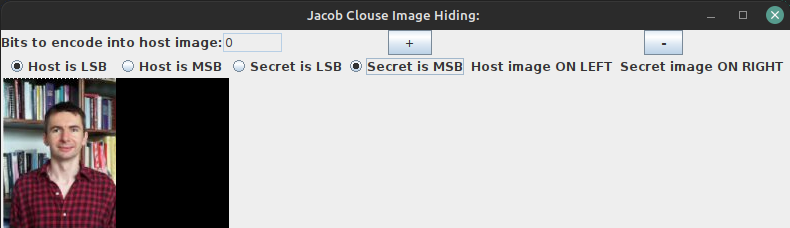
\includegraphics[scale=.7]{default_0.png}\\
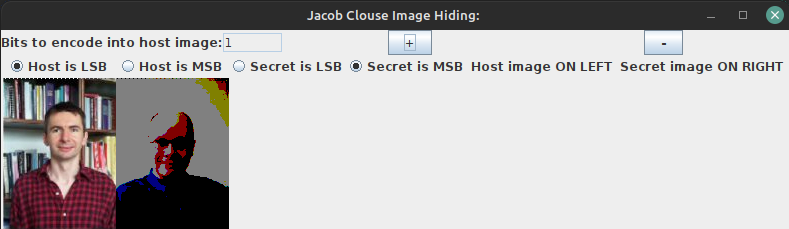
\includegraphics[scale=.7]{default_1.png}\\
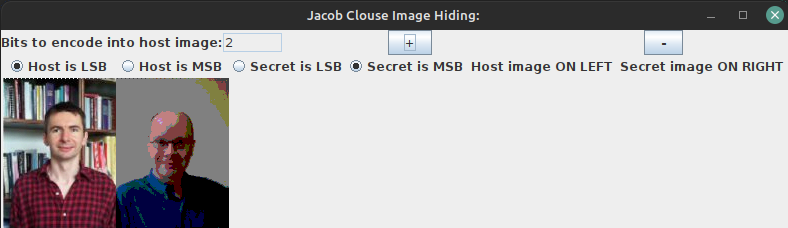
\includegraphics[scale=.7]{default_2.png}\\
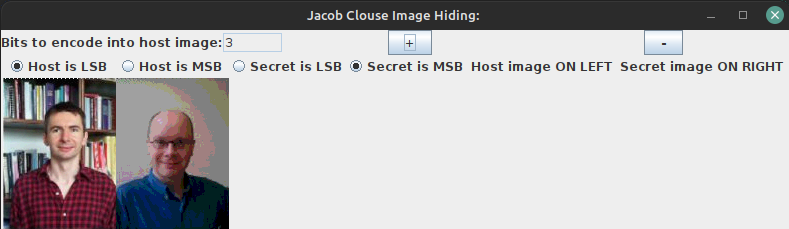
\includegraphics[scale=.7]{default_3.png}\\
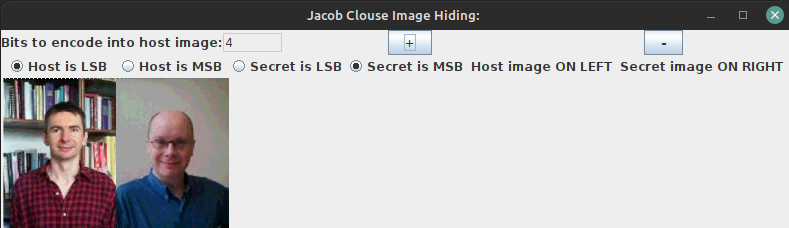
\includegraphics[scale=.7]{default_4.png}\\
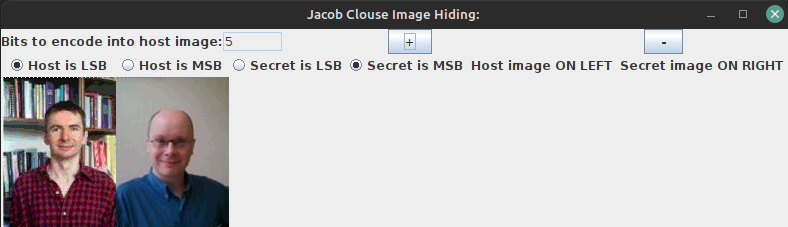
\includegraphics[scale=.7]{default_5.png}\\
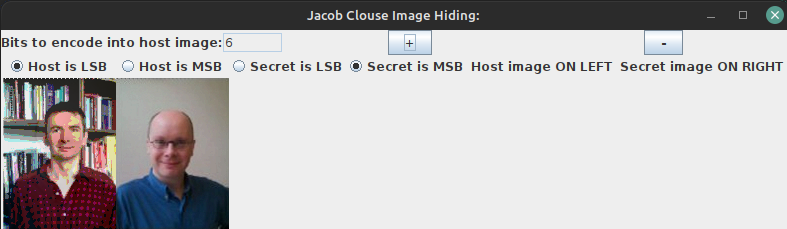
\includegraphics[scale=.7]{default_6.png}\\
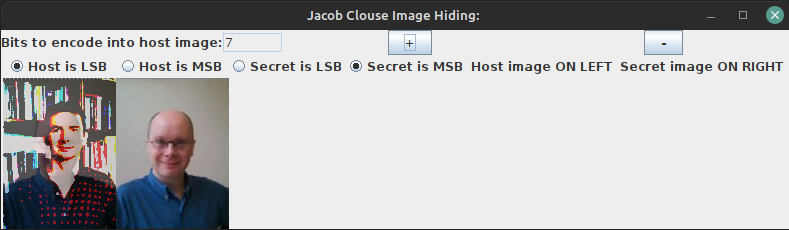
\includegraphics[scale=.7]{default_7.png}\\
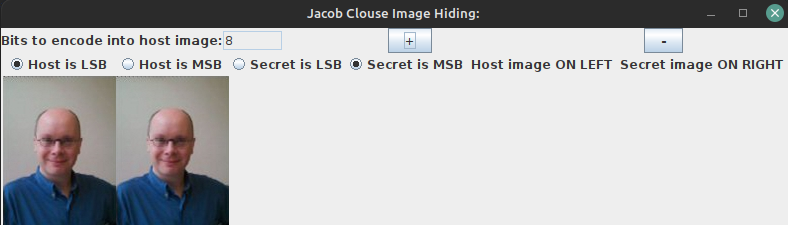
\includegraphics[scale=.7]{default_8.png}\\
\vspace{0.2in} \\
But when we reversed and instead hide the LSB of the Secret Image in the MSB of the Host Image, we get results that are not recognizable until past the halfway point. The colors are cooler in the Secret Image as well:\\
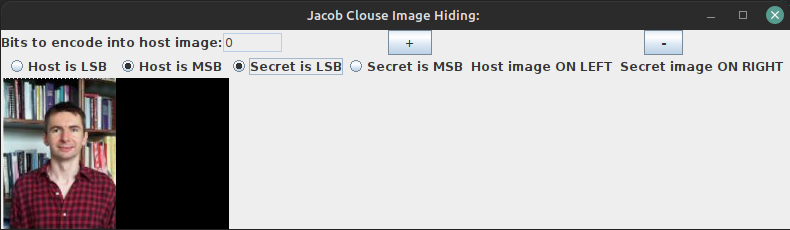
\includegraphics[scale=.7]{opp_0.png}\\
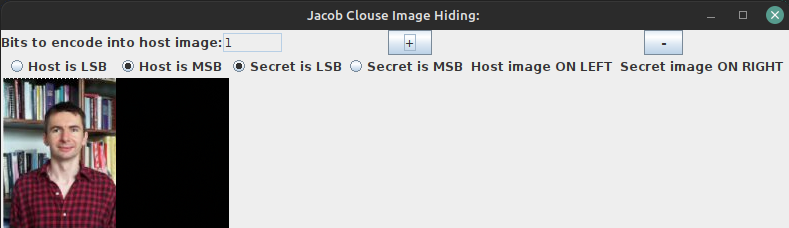
\includegraphics[scale=.7]{opp_1.png}\\
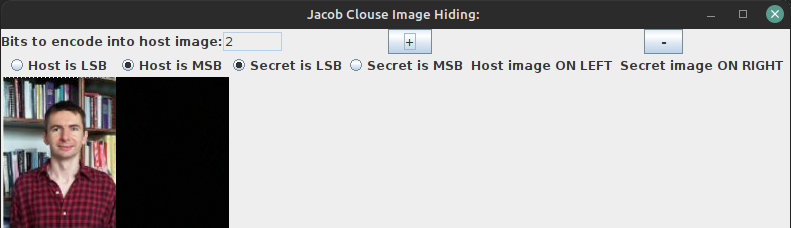
\includegraphics[scale=.7]{opp_2.png}\\
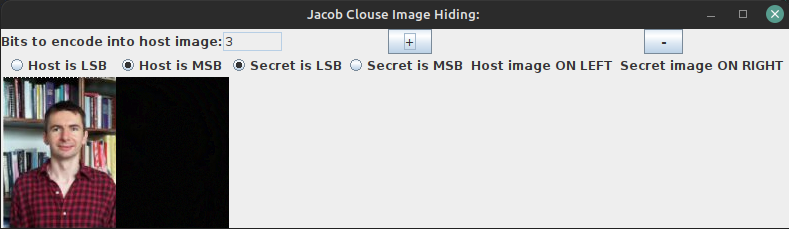
\includegraphics[scale=.7]{opp_3.png}\\
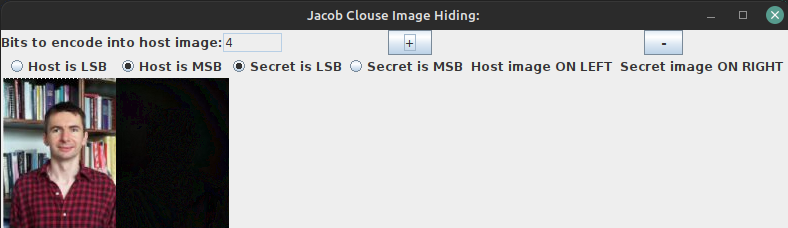
\includegraphics[scale=.7]{opp_4.png}\\
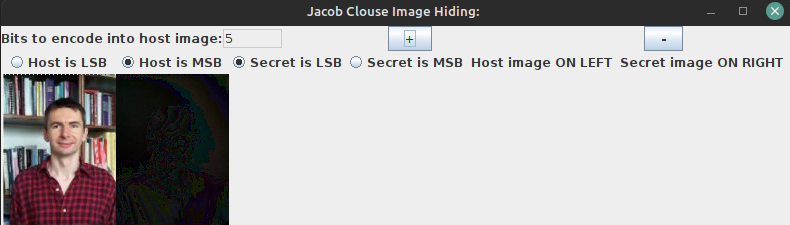
\includegraphics[scale=.7]{opp_5.png}\\
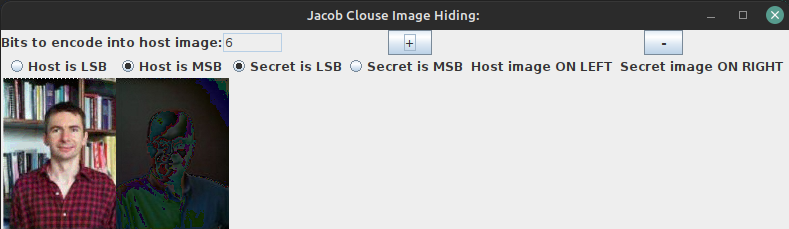
\includegraphics[scale=.7]{opp_6.png}\\
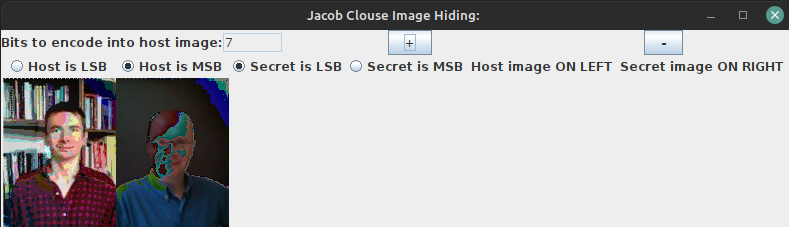
\includegraphics[scale=.7]{opp_7.png}\\
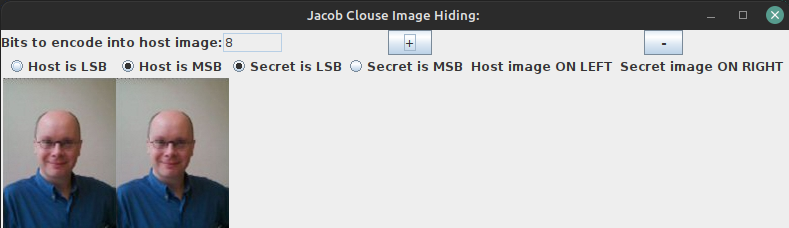
\includegraphics[scale=.7]{opp_8.png}\\



\fi
\end{document}